\section{Experiments}

%
% NOTE: figures are named <experimentsection>_<subsection>_<xaxis>.pdf
%

\subsection{Setup}


We run a mix of synthetic and real world experiments.

\subsubsection{Dataset and Workload}

Anant's workload?

Synthetic dataset.


\subsubsection{Generating Complaints and Complaint Sets}



\subsubsection{Metrics}

\begin{itemize}
\item Percentage of complaints correctly modified
\item Percentage of errors introduced
\item Execution time
\item Distance from corrected modification (str distance, clause distance, numerical distance)
\end{itemize}

\subsubsection{Comparison}

\begin{itemize}
\item Query By Example algorithm
\item Quoc's ConQueR
\end{itemize}

Conditions:

\begin{itemize}
\item {\bf NQueries:} Vary number of queries in the query log
\item {\bf DBSize: } Size of the database (number of tuples)
\item {\bf NClauses:} The number of clauses in the where conditions.
\item {\bf ErrDim: } Number of attributes that 
\item {\bf ErrIdx: } The index of the query in the query log that was corrupted.
\item {\bf CSPerc: } Percentage of true complaint set was selected as input.
\item {\bf FPPerc: } Percentage of false positives in the complaint set.
\end{itemize}


\subsection{Single-Query Log}

In the first set of experiments, we evaluate the simplest case where there
is a single update query.  In each experiment, we vary the DBSize,
NClauses, as well as the number of clauses in the query that have
been corrupted and report the metrics described above.  We first 
compare the learning algorithms on a complete complaint set, then evaluate them
using incomplete complaint sets with varying percentages of false positive and negative complaints.

\subsubsection{Complete Complaints}

Vary DBSize

Vary NClauses, corrupt 1 and 2 clauses

We found that CPLEX and BBOX identify the correct fix, however their
running times are significantly higher than DTree.  This is because
CPLEX is an exact solution, as compared to DTree, whose poor early
splitting decisions can adversely affect the final tree structure.

\subsubsection{Incomplete Complaints}


Vary DBSize

Vary NClauses, corrupt 1 and 2 clauses

Each line varies perc FP

We first increased the number of false positives in the complaint set (no false negatives).
Figure~\ref{f:single_incomplete_fp} shows how the fix quality and running time vary as the
percentage of false positives increases.   Compared variations of CPlex and Bounding box with varying
density thresholds (?).

Each line varies perc FN

We then varied the number of false negatives while keeping the percentage of false positives fixed at 5\%.
Figure~\ref{f:single_incomplete_fn} 


\subsection{Increased Query Log Size}

In the following set of experiments, we increase the number of
queries in the log while varying ?.  The number of corrupted queries
is still one.  In these experiments, we set the DBSize to 10000,
the default NClauses to 4, and the number of corrupted clauses to
2.   We first show results for varying the false positives and
negatives in the complaint set and comparing the algorithms described
in Section~\ref{s:incomplete-algs}.  We then evaluate the efficacy
of of provenance-based query log filtering, which reduces the running
time without affecting the result quality.

To generate the false-positive data

\subsection{False Positive}

Vary false positives (1 graph)

\subsection{False Negative}

Vary false negatives (1 graph)

\subsubsection{Filtering Queries}

We also compared the provenance-based filtering techniques in the above experiments
to measure their effectiveness at reducing the running time.  We varied the complexity of the update 
WHERE clauses to control the amount that queries in the log overlap in their updates.  The query log contained 50 update WHERE queries.
The quality of the suggested fixes were the same,  As the clauses became less complex, the likelihood 
of overlap increased, and increased the amount of queries that affected the complaint sets.


\begin{figure}[h]
\centering
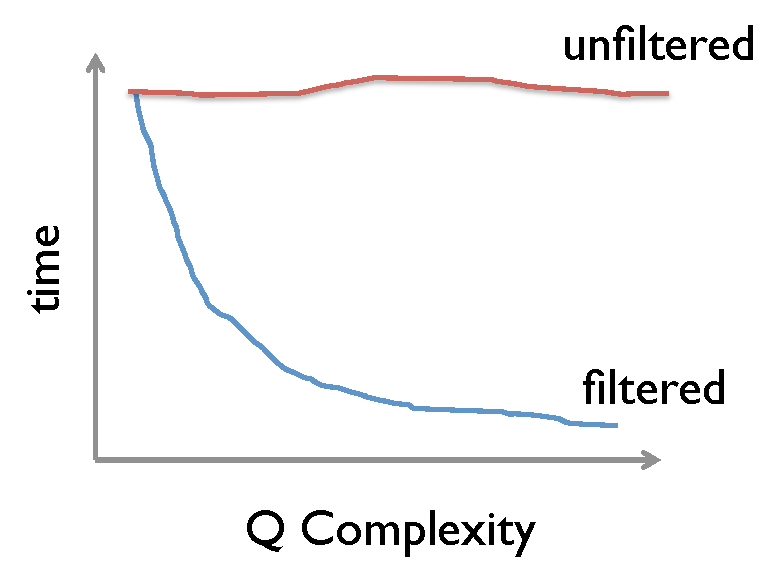
\includegraphics[width = 2in]{figures/complete_qfilter_complexity}
\caption{Varying query complexity.}
\label{f:complete_qfilter_complexity} 
\end{figure}



\subsection{Multi-Query}

Using a previous experimental configuration, we varied the number of queries that are corrupted.  Figures~\ref{}
show the quality and running times of the results for a query log of size 1000 and dbsize of 100k.  
As we can see, the cost increases quadratically with each corrupted query and the accuracy of the proposed fixes increases marginally.  
This is because XXX.


To better understand the algorithm, we plot the quality metrics after each fixed query and measure how quickly \sys converges to the final result. 
This suggests that an incremental approach where the user can set a threshold to stop the algorithm may be effective.


\subsection{Real Transactional Workload}

We used the web application workload, and evaluated our alogirthms with artifically injected corruptions.
We compared two types of corruptinos.  In figure~\ref{f:real_existing}, we randomly picked a single existing 
query and corrupted its value.  If the query was an INSERT, we randomly pick a value and perturbed it.
If the transaction was an UPDAET, we randomly varied the SET or WHERE clauses.   We re-ran this
100 times and plot the average and standard deviation of the results.

